\chapter{The Lagrangian as a Code for Field Equations and Interactions}

These notes follow Leonard Susskind's Lecture 9 in \emph{Particle Physics 1: Basic Concepts}, with curation by LazyingArt LLC. The lecture opens with a simple but important dissatisfaction. Every field has an equation of motion, but merely listing those equations one by one is a clumsy way to organize the physics. The Lagrangian is introduced as the compact object that does the whole job at once. First it generates the classical field equations. Then, when the same symbols are read as quantum fields, it becomes a code for local processes of propagation, emission, absorption, creation, annihilation, and scattering.

\section{Why Field Equations Are Coded by a Lagrangian}

Boson fields, fermion fields, and electromagnetic fields all satisfy wave-like equations involving time derivatives, space derivatives, and the field itself. One could certainly write those equations down individually, and the lecture says so explicitly. But that is only the crude description. The more powerful statement is that there is a single compact expression from which all the equations of motion of the system follow.

That expression is the Lagrangian. Susskind mentions its relation to the principle of least action, but does not rederive that principle here. He wants instead to remind us of the operational content: what the Lagrangian depends on, how it generates field equations, and why the same formalism later acquires a new meaning in quantum field theory. Already at the beginning, then, the Lagrangian is not presented as one more formula. It is presented as a code.

\begin{figure}[htbp]
\centering

\includegraphics[width=0.82\textwidth]{lecture_09_figure_03.png}
\caption{Lagrangian as a function of fields and derivatives}
\end{figure}

For a single scalar field, the board writes
\begin{equation}
\mathcal{L}
=
\mathcal{L}\!\left(\phi,\partial_t\phi,\partial_x\phi,\ldots\right)
=
\mathcal{L}\!\left(\phi,\partial_\mu\phi\right).
\end{equation}
That one line already carries the pedagogical move of the lecture. We begin with explicit time and space derivatives, and only then compress them into the relativistic shorthand \(\partial_\mu\phi\). The notation is being organized as the physics is being organized.

\section{One Scalar Field: Dependence and the Euler--Lagrange Rule}

Having written what \(\mathcal L\) depends on, the lecture immediately asks what we do with it. The answer is given without proof. He says in so many words: we are not going to argue for these equations now; we are simply going to use them.

For one field \(\phi\), the field-theory Euler--Lagrange equation is
\begin{equation}
\frac{\partial}{\partial t}\frac{\partial \mathcal L}{\partial \dot\phi}
+
\frac{\partial}{\partial x}\frac{\partial \mathcal L}{\partial \phi_x}
+
\frac{\partial}{\partial y}\frac{\partial \mathcal L}{\partial \phi_y}
+
\frac{\partial}{\partial z}\frac{\partial \mathcal L}{\partial \phi_z}
=
\frac{\partial \mathcal L}{\partial \phi},
\end{equation}
where
\[
\dot\phi=\frac{\partial \phi}{\partial t},
\qquad
\phi_x=\frac{\partial \phi}{\partial x},
\qquad
\phi_y=\frac{\partial \phi}{\partial y},
\qquad
\phi_z=\frac{\partial \phi}{\partial z}.
\]

He then narrows at once to the simplest scalar field. Its Lagrangian is
\begin{equation}
\mathcal L
=
\frac12 \dot\phi^{\,2}
-
\frac12 (\nabla\phi)^2
-
V(\phi).
\end{equation}
The undifferentiated field enters only through the potential \(V(\phi)\). This is precisely the visual point made on the board: the potential term sits at the right edge and anchors the whole example.

\begin{figure}[htbp]
\centering

\includegraphics[width=0.72\textwidth]{lecture_09_figure_04.png}
\caption{Potential term in the scalar-field Lagrangian}
\end{figure}

The frame shows only the right half of the board, so the typeset equations below are a cautious standard completion of what is only partly visible in the screenshot. Still, the board layout matters: first the general rule, then the concrete scalar Lagrangian, then the resulting field equation.

We compute
\begin{align}
\frac{\partial \mathcal L}{\partial \dot\phi} &= \dot\phi,
&
\frac{\partial \mathcal L}{\partial \phi_x} &= -\phi_x,
&
\frac{\partial \mathcal L}{\partial \phi_y} &= -\phi_y,
&
\frac{\partial \mathcal L}{\partial \phi_z} &= -\phi_z,
\\
\frac{\partial \mathcal L}{\partial \phi} &= -\frac{\partial V}{\partial \phi}.
\end{align}
Therefore
\begin{equation}
\ddot\phi-\nabla^2\phi=-\frac{\partial V}{\partial \phi}.
\end{equation}

At this stage the lecture is still deliberately elementary. It is not trying to impress us with formal machinery. It is showing us, in the cleanest possible example, how the code is decoded.

There is also a familiar classical pattern sitting inside the formula:
\[
\mathcal L = \text{kinetic structure} - \text{potential energy}.
\]
Later in the lecture he returns to this explicitly: time derivatives play the role of kinetic energy, and undifferentiated field terms play the role of potential energy, just as they do in ordinary mechanics.

\section{Scalar Example: Mass Term, Wave Equation, and Relativistic Dispersion}

Now the lecture asks what choices of \(V(\phi)\) are interesting. A constant is uninteresting, since its derivative vanishes. A linear function is possible algebraically, but physically unstable, because the potential would be unbounded below. So the first genuinely useful example is
\begin{equation}
V(\phi)=\frac12 m^2\phi^2.
\end{equation}
Then
\begin{equation}
\frac{\partial V}{\partial\phi}=m^2\phi,
\end{equation}
and the field equation becomes
\begin{equation}
\ddot\phi-\nabla^2\phi=-m^2\phi.
\end{equation}

This is where the lecture takes its first real payoff. We do not leave the equation sitting there as formal symbolism. We ask what it says about the quanta of the field. Take a plane wave of the form
\begin{equation}
\phi(\mathbf x,t)\sim e^{i\omega t-i\mathbf k\cdot\mathbf x}.
\end{equation}
Two time derivatives give
\[
\ddot\phi = -\omega^2\phi,
\]
while the Laplacian gives
\[
\nabla^2\phi = -k^2\phi,
\qquad
k^2=\mathbf k\cdot\mathbf k.
\]
Substituting into the wave equation,
\begin{equation}
-\omega^2\phi-(-k^2)\phi=-m^2\phi.
\end{equation}
Canceling the common factor \(\phi\), we obtain
\begin{equation}
\omega^2-k^2=m^2,
\end{equation}
or, more suggestively,
\begin{equation}
\omega^2=k^2+m^2.
\end{equation}
In units with \(\hbar=c=1\), this is exactly
\begin{equation}
E^2=p^2+m^2.
\end{equation}

So the coefficient \(m\) in the potential is not merely a convenient parameter. It is the mass of a single quantum of the field. That is the content of the wave equation.

The lecture inserts one more point here, and it is a good one to insert here. If we want relativistic equations in the end, then the Lagrangian itself must be a scalar under Lorentz transformations. The spatial minus signs are not an afterthought. They are the field-theory version of the relativistic sign difference between space and time.

\section{Nonlinearity, Multiple Fields, and Classical Scattering}

Once the free scalar field has been understood, the lecture turns to interaction by the simplest possible move: increase the power of the field. Suppose
\begin{equation}
V(\phi)\supset g\phi^3.
\end{equation}
Then
\begin{equation}
-\frac{\partial}{\partial \phi}(g\phi^3)=-3g\phi^2,
\end{equation}
so the equation of motion becomes
\begin{equation}
\ddot\phi-\nabla^2\phi=-m^2\phi-3g\phi^2.
\end{equation}

Now the equation is no longer linear. That is the crucial change. For a linear equation, if one wave packet moves one way and another wave packet moves the other way, their sum is still a solution. They interfere while they overlap, but afterwards they emerge undeformed. Once the equation is nonlinear, that superposition principle fails. The wave packets affect one another, scatter, distort, and can in principle do much more complicated things. In the lecture this is the first classical meaning of interaction.

The same point becomes sharper if we introduce two fields. Let \(\phi\) and \(\rho\) be two scalar fields and write
\begin{align}
\mathcal L
&=
\frac12 (\partial_\mu\phi)^2
+
\frac12 (\partial_\mu\rho)^2
-
V(\phi,\rho),
\\
V(\phi,\rho)
&=
\frac12 m^2\phi^2+\frac12 M^2\rho^2+\rho\phi^2.
\end{align}
If the mixed term \(\rho\phi^2\) were absent, then the fields would decouple:
\begin{equation}
\ddot\phi-\nabla^2\phi=-m^2\phi,
\qquad
\ddot\rho-\nabla^2\rho=-M^2\rho.
\end{equation}
That would describe two independent kinds of quanta, with masses \(m\) and \(M\).

But once the mixed term is present, we have
\begin{align}
\ddot\phi-\nabla^2\phi &= -m^2\phi-2\rho\phi,
\\
\ddot\rho-\nabla^2\rho &= -M^2\rho-\phi^2.
\end{align}
Now each equation contains the other field. The system is coupled, and because the mixed term is not quadratic, it is nonlinear as well. A wave packet of \(\phi\) can scatter a wave packet of \(\rho\), and a wave packet of \(\rho\) can scatter a wave packet of \(\phi\).

The lecture is very explicit about what the terms mean. The derivative terms tell us about energy and momentum. The quadratic field term tells us about mass. The higher-order mixed term tells us about interaction between quanta. That is classical field theory in a nutshell.

\section{Dirac Field and Scalar--Fermion Coupling}

The next example is the Dirac field. The lecture is intentionally informal here. Susskind says outright that he does not quite remember where all the \(i\)'s go. That admission matters, because it tells us how the section is to be read: not as a polished derivation, but as a bridge. He wants to show that the same pattern survives the move from scalar fields to fermions.

The board writes the Dirac equation in one-dimensional shorthand as
\begin{equation}
i\dot\Psi=i\alpha\frac{\partial\Psi}{\partial x}+m\beta\Psi.
\end{equation}
As he immediately says, this really abbreviates the full spatial structure
\begin{equation}
i\dot\Psi=i\sum_i \alpha_i\frac{\partial\Psi}{\partial x_i}+m\beta\Psi.
\end{equation}
The \(\alpha_i\) and \(\beta\) are Dirac matrices, so the field is now multi-component, but the conceptual point is unchanged: there is again an equation of motion, and there is again a Lagrangian that generates it.

\begin{figure}[htbp]
\centering

\includegraphics[width=0.76\textwidth]{lecture_09_figure_05.png}
\caption{Dirac equation and its Lagrangian}
\end{figure}

A cleaned version, close to both the transcript and the finished board state, is
\begin{equation}
\mathcal L_{\mathrm D}
\sim
i\left(
\Psi^\dagger \frac{\partial\Psi}{\partial t}
+
\Psi^\dagger \alpha \frac{\partial\Psi}{\partial x}
+
m\Psi^\dagger\beta\Psi
\right).
\end{equation}
This formula should be read with caution. The lecture does not ask us to canonize every chalk mark. It asks us to register the structure: the Dirac field too is encoded in a Lagrangian.

Now suppose we also have a scalar boson field \(\phi\). We can then couple the two fields together. The lecture first writes a term that is not Lorentz invariant, then repairs it by inserting a \(\beta\). The cleaned lecture-facing form is
\begin{equation}
\mathcal L_{\mathrm{int}}\propto \Psi^\dagger\beta\Psi\,\phi.
\end{equation}
This is enough for the point at hand. The scalar field can scatter the Dirac field, and the Dirac field can scatter the scalar field. If we varied the full Lagrangian, we would obtain a Dirac equation with an extra term proportional to \(\phi\), and a scalar field equation with an extra term involving the fermion bilinear.

He then makes a suggestive remark. Compare
\begin{equation}
m\Psi^\dagger\beta\Psi
\qquad\text{with}\qquad
\Psi^\dagger\beta\Psi\,\phi.
\end{equation}
It is almost as though the mass parameter \(m\) had been replaced by a scalar field. The lecture does not develop this yet, but it plants the seed for the Higgs-like coda at the end.

At this point the classical story is finished. Classical wave packets scatter other classical wave packets. What about quantum field theory?

\section{From Field Operators to QED Vertices}

Now the ontology changes without the algebra changing very much. The fields are no longer to be thought of as classical waves. They are operator-valued objects built from creation and annihilation operators. That is the major pivot of the lecture.

Start with a scalar field. Schematically,
\begin{equation}
\phi \sim A^+ + A^-,
\end{equation}
where \(A^+\) creates quanta and \(A^-\) annihilates them. Then \(\phi^3(x)\) contains a whole list of local processes at the same point \(x\):
\begin{itemize}
\item one particle in and two out;
\item two particles in and one out;
\item three particles created at a point;
\item three particles annihilated at a point.
\end{itemize}
So the cubic term that classically produced nonlinearity now becomes a local code for quantum processes.

The Dirac field is slightly subtler, because it contains both electron and positron content. The lecture goes through the historical language of positive and negative energies, and then uses the standard reinterpretation: removing a negative-energy electron is the same as creating a positive-energy positron. In that language,
\begin{align}
\Psi &\sim C^-_{\text{electron}}(+E)+C^+_{\text{positron}}(+E),
\\
\Psi^\dagger &\sim C^+_{\text{electron}}(+E)+C^-_{\text{positron}}(+E).
\end{align}
These expressions are schematic on purpose. The board is partly obscured, and the lecture itself is not trying to give a full normalized mode expansion. What matters is the operator content: \(\Psi\) annihilates electrons and creates positrons, while \(\Psi^\dagger\) does the reverse.

A useful technical remark from the discussion belongs here. When derivatives appear in the equations, one does \emph{not} differentiate the creation or annihilation operators themselves. The field is expanded as operators multiplying plane-wave factors such as \(e^{i\mathbf k\cdot \mathbf x-i\omega t}\), and the derivatives act on those exponentials, pulling down factors of \(k\) and \(\omega\). The operators are, in that sense, like coefficients in the spacetime expansion.

The canonical example is then quantum electrodynamics. The basic interaction is written in the lecture's mixed time-space notation as
\begin{equation}
\mathcal L_{\mathrm{QED,int}}
=
e\left(\Psi^\dagger\Psi\,A_0+\Psi^\dagger\alpha\Psi\cdot\mathbf A\right).
\end{equation}
Here \(A_0\) and \(\mathbf A\) are the time and space components of the electromagnetic vector potential. The lecture pauses to justify the scalar nature of this expression: \(A_\mu\) is a vector, so we must pair it with a vector built from the Dirac field. In this notation, \(\Psi^\dagger\Psi\) is the time component and \(\Psi^\dagger\alpha\Psi\) the spatial component.

\begin{figure}[htbp]
\centering

\includegraphics[width=0.78\textwidth]{lecture_09_figure_06.png}
\caption{Field-operator decomposition and photon-emission sketch}
\end{figure}

Because the photon field also contains creation and annihilation operators, one local term now contains a whole family of possible readings. Multiplying out the operator content of \(\Psi^\dagger\), \(\Psi\), and \(A\), we find:
\begin{itemize}
\item an electron emits a photon;
\item an electron absorbs a photon;
\item an electron and a positron annihilate into a photon;
\item a photon creates an electron-positron pair.
\end{itemize}
The lecture's delight at this point is worth preserving. One simple local term describes all these different processes. It is quite remarkable.

The screenshot is mainly a witness to the classroom staging of this idea. The left side of the board holds the schematic \(\Psi\) and \(\Psi^\dagger\) decompositions; the lower middle hides part of the interaction formula; the right side shows the wavy photon sketch. The cleaned redraw below is only an interpretation of that discussion, not a replacement for it.

\begin{figure}[htbp]
\centering
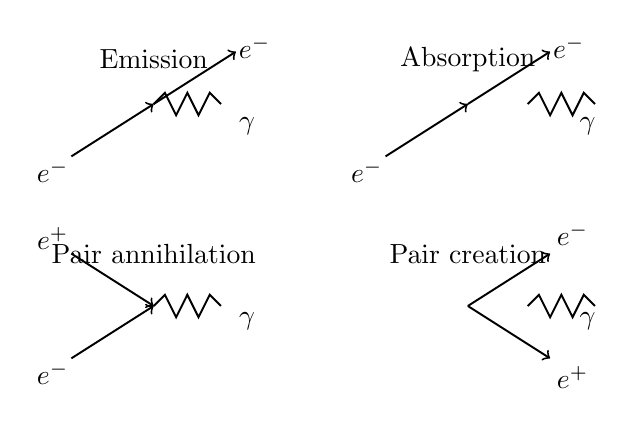
\begin{tikzpicture}[line width=0.7pt, scale=0.95]
\node at (1.2,4.2) {Emission};
\draw[->] (0.1,2.9) -- (1.2,3.6);
\draw[->] (1.2,3.6) -- (2.3,4.3);
\draw (1.2,3.6)--(1.35,3.75)--(1.5,3.45)--(1.65,3.75)--(1.8,3.45)--(1.95,3.75)--(2.1,3.6);
\node at (-0.15,2.7) {$e^-$};
\node at (2.55,4.35) {$e^-$};
\node at (2.45,3.3) {$\gamma$};

\node at (5.4,4.2) {Absorption};
\draw[->] (4.3,2.9) -- (5.4,3.6);
\draw[->] (5.4,3.6) -- (6.5,4.3);
\draw (7.1,3.6)--(6.95,3.75)--(6.8,3.45)--(6.65,3.75)--(6.5,3.45)--(6.35,3.75)--(6.2,3.6);
\node at (4.05,2.7) {$e^-$};
\node at (6.75,4.35) {$e^-$};
\node at (7.0,3.3) {$\gamma$};

\node at (1.2,1.6) {Pair annihilation};
\draw[->] (0.1,0.2) -- (1.2,0.9);
\draw[->] (0.1,1.6) -- (1.2,0.9);
\draw (1.2,0.9)--(1.35,1.05)--(1.5,0.75)--(1.65,1.05)--(1.8,0.75)--(1.95,1.05)--(2.1,0.9);
\node at (-0.15,0.0) {$e^-$};
\node at (-0.15,1.8) {$e^+$};
\node at (2.45,0.7) {$\gamma$};

\node at (5.4,1.6) {Pair creation};
\draw (7.1,0.9)--(6.95,1.05)--(6.8,0.75)--(6.65,1.05)--(6.5,0.75)--(6.35,1.05)--(6.2,0.9);
\draw[->] (5.4,0.9) -- (6.5,1.6);
\draw[->] (5.4,0.9) -- (6.5,0.2);
\node at (7.0,0.7) {$\gamma$};
\node at (6.8,1.85) {$e^-$};
\node at (6.8,-0.05) {$e^+$};
\end{tikzpicture}
\caption{A schematic redraw of the QED vertex family. The arrows indicate charge flow schematically. The lecture's point is that one local interaction can be read as emission, absorption, pair annihilation, or pair creation by rotating the legs.}
\end{figure}

All these processes come with the same coefficient \(e\). The lecture identifies that coefficient as the electric charge of the electron. In these microscopic units it is dimensionless, and its physical meaning is quantum-mechanical: \(e\) is the amplitude for the basic QED vertex, so \(e^2\) sets the corresponding probability scale. He even gives the concrete picture of an electron stopped abruptly at a wall; the probability that its momentum continues off as a photon is governed by \(e^2\).

The operators in the basic QED vertex are all evaluated at the same spacetime point. At the elementary level there is no delay built into the process: the electron is absorbed, re-emitted, and the photon emitted or absorbed at one point.

Charge conservation appears twice over. Diagrammatically, the fermion arrows must go through the vertex continuously. Algebraically, the interaction contains one \(\Psi\) and one \(\Psi^\dagger\), so the charge increase produced by one is canceled by the charge decrease produced by the other.

\subsection{Question \& Answer}

\paragraph{Question.}
If one local QED vertex can be rotated in so many ways, why do some of the resulting pictures seem to describe impossible processes, such as an electron, a positron, and a photon all disappearing into nothing?

\paragraph{Answer.}
Because the local vertex is not yet the full physical amplitude. It is only the elementary process at a single spacetime point. To obtain a real amplitude one must integrate over all the places and times at which that elementary process could occur. Those spacetime integrals enforce momentum conservation and energy conservation. Once that is done, the kinematically forbidden pictures simply drop out. So the local vertex allows more pictures than nature finally permits; the spacetime integrals impose the final constraints.

\section{Locality, Repeated Action, Symmetry, and the Size of the Full Theory}

The lecture now turns back to the quadratic terms and asks for their quantum meaning. A derivative can be thought of as a difference between neighboring points:
\begin{equation}
\partial_x\phi(x)\sim \frac{\phi(x)-\phi(x')}{L},
\end{equation}
where \(x'\) is close to \(x\) and \(L\) is the separation. Thus
\begin{equation}
\frac12\bigl(\partial_x\phi\bigr)^2
\sim
\frac{1}{2L^2}\bigl[\phi(x)-\phi(x')\bigr]^2.
\end{equation}
The same-point pieces simply absorb and re-emit a particle at one location. The cross-term connects the neighboring points \(x\) and \(x'\). In the lecture's language, it removes a particle from one point and makes it reappear at the other. That is how the quadratic derivative terms govern the motion of an undisturbed particle.

The mass term
\begin{equation}
\frac12 m^2\phi^2
\end{equation}
is similar to the same-point part of the derivative term, not to the hopping part. It does not move the particle. It acts at one point, absorbing and re-emitting it there. One can also say, more passively, that it counts or weights the presence of the particle at that point. In either reading, it is local and non-transporting.

\subsection{Question \& Answer}

\paragraph{Question.}
How can a strictly local Lagrangian describe something extended, such as a proton here exchanging a photon with an electron there?

\paragraph{Answer.}
Because there is no single term in the Lagrangian for the whole long-distance exchange. The exchange is built from many local pieces. One local term emits the photon. Quadratic terms move it from neighboring point to neighboring point. Another local term absorbs it. If we divide space or spacetime into little cells, then the fields live on those cells and the quadratic terms hop particles from one cell to the next. The continuum theory is the limit in which the cell size goes to zero. So there is no action at a distance. There are only local interactions and infinitesimal steps.

This discrete-cell picture is important in the lecture. In classical physics one often defines derivatives by differences and then forgets the discreteness. Here the point is a little sharper: quantum field theory is to be thought of as built from local cells, with the continuum recovered as a limit. Motion becomes hopping. Local interaction remains local interaction.

From there the lecture gives a heuristic combinatorial rule for repeated local action. One writes, schematically,
\begin{equation}
\prod_x \bigl(1+\mathcal L_I(x)\bigr),
\end{equation}
where \(\mathcal L_I(x)\) is the interaction Lagrangian at the spacetime point \(x\). He says explicitly that this is a trick and that he is cheating a little. But it is a very useful trick, because it generates all combinations of local processes. For two points,
\begin{equation}
(1+\mathcal L_I(x))(1+\mathcal L_I(x'))
=
1+\mathcal L_I(x)+\mathcal L_I(x')+\mathcal L_I(x)\mathcal L_I(x').
\end{equation}
The first term means nothing happens. The next two mean one local interaction occurs at one point or the other. The last term means both local interactions occur. Multiply enough such factors together and one generates amplitudes built from basic local units in all possible ways.

This is also how the lecture answers questions about more complicated processes. A proton emitting a photon and an electron later absorbing it is not described by one special nonlocal term. It is described by the product of local emission, many local propagation steps, and local absorption. The amplitude is the sum over all such allowed ways of getting from the initial state to the final state.

Initial and final conditions then fit naturally into the same picture. One starts from the vacuum, creates the incoming particles at the source points, lets the Lagrangian act repeatedly in between, and annihilates the outgoing particles at the detector points. What the sources prepare and what the detectors absorb are not the whole theory; what happens in between is governed by the repeated action of the Lagrangian.

At this stage the lecture broadens from dynamics to symmetry. A basic example is the global phase transformation
\begin{equation}
\Psi \to e^{i\theta}\Psi,
\qquad
\Psi^\dagger \to e^{-i\theta}\Psi^\dagger,
\qquad
A \to A.
\end{equation}
Because the interaction contains equal numbers of \(\Psi\) and \(\Psi^\dagger\), it is invariant under this transformation. The lecture reads this immediately as charge conservation. This is one of the great uses of the Lagrangian formalism: once the terms are written down, we can read off symmetries, and from symmetries we can read off conservation laws.

As a short effective-field coda, the lecture turns to protons, neutrons, and pions. The original discussion includes a live correction of charge assignment, so we keep only the corrected charge-conserving form. Effective vertices such as
\begin{equation}
\Psi_p^\dagger\Psi_n\,\pi^+,
\qquad
\Psi_n^\dagger\Psi_p\,\pi^-,
\qquad
\Psi_p^\dagger\Psi_p\,\pi^0,
\qquad
\Psi_n^\dagger\Psi_n\,\pi^0
\end{equation}
encode many charge-conserving nucleon-pion processes. Because the proton is charged, one also has the proton-photon vertex
\begin{equation}
\Psi_p^\dagger\Psi_p\,A.
\end{equation}
The lesson is the same as in QED. A small number of local terms yields a large family of allowed processes once the legs are reinterpreted and rotated appropriately.

The lecture then steps back even further. There is, at least in the physicist's working picture, one enormous Lagrangian containing many fields and many coupling constants. The art is in figuring out what that Lagrangian is from experimental data. Once it is known, the rules for calculating amplitudes are precise. But it is not a pretty picture. One usually works with a manageable sector of the whole thing, because many parts of the full theory are irrelevant at a given scale. In that sense quantum field theory feels exact and phenomenological at once: exact in method, phenomenological in the form of the effective Lagrangian one actually uses.

A final sketch points toward the Higgs mechanism. Suppose a field \(H\) enters through a term
\begin{equation}
\mathcal L \supset H\phi^2 - V(H).
\end{equation}
Since \(H\phi^2\) is cubic, it describes a \(\phi\) in, a \(\phi\) out, and an \(H\) emitted. But now imagine that the potential \(V(H)\) has minima away from the origin, so that the vacuum settles at
\begin{equation}
\langle H\rangle \neq 0.
\end{equation}
Then the factor \(H\) in the cubic vertex can be replaced, in the vacuum, by a number. In that way the interaction begins to look like an effective quadratic mass term. The lecture only sketches this and does not try to give a full development, but the intended idea is clear.

\section{Summary}

The lecture unfolds one idea step by step. The Lagrangian is a compact code for the dynamics of fields. In classical field theory it generates equations of motion; in quantum field theory it encodes local particle processes. Quadratic terms describe free propagation and mass, higher-order terms describe interaction, spacetime integration restores energy-momentum conservation, and symmetries of the Lagrangian become conservation laws. Extended processes are not built from action at a distance, but from repeated local steps. The picture is at once simple and wide: one writes down a Lagrangian, and from it one reads equations, vertices, amplitudes, symmetries, and, ultimately, a large part of the structure of particle physics.